\clearpage
\appendix
\section{Resoconto attività di verifica}
\label{sec:resoconto}
\subsection{Revisione dei Requisiti}
\label{sec:revisione_requisiti}
\subsubsection{Qualità di processo}
Nella presente sezione, si riassumono gli esiti delle attività di verifica svolte sui documenti consegnati nelle varie revisioni di progetto, e sul prodotto software in sviluppo.
\subsubsection{Qualità di prodotto}
In questa fase del progetto le metriche di prodotto istanziate sono quelle riguardanti i documenti.
\paragraph{MPRDD001 - Indice di Gulpease}\mbox{}\\[0.4cm]
Per mezzo di script automatici è stato possibile istanziare la metrica  \textbf{MPRDD001 Indice di Gulpease}.\\
Nella tabella sottostante è mostrato il risultato ottenuto per i principali documenti prodotti.
\begin{center}
	\centering
	\renewcommand{\arraystretch}{1.5}
	\rowcolors{3}{tableLightYellow}{}
	\begin{longtable}{  p{5cm}  p{5cm} p{3cm}  }
		\rowcolor{tableHeadYellow}
		\textbf{Nome documento}   & \textbf{Indice di \mbox{Gulpease}} & \textbf{Esito} \\ 
		\endhead
		Studio di Fattibilità     & 89                                 & Ottimo \\
		Norme di Progetto         & 97                                 & Ottimo \\
		Analisi dei Requisiti     & 80                                 & Ottimo \\
		Piano di Progetto         & 100                                & Ottimo \\
		Piano di Qualifica        & 96                                 & Ottimo \\
		\rowcolor{white}
		\caption{Resoconto misurazioni metrica MPRDD001 - Indice di Gulpease}
	\end{longtable}
\end{center}
\paragraph{MPRDD002 - Errori ortografici}\mbox{}\\[0.4cm]
Tutti i documenti, dopo un rigoroso controllo da parte dei verificatori ed un feedback positivo rilasciato dallo strumento di controllo della sintassi di TexStudio, risultano privi di errori e raggiungono il valore accettabile ed ottimale della metrica  \textbf{MPRDD002 Correttezza ortografica}.

\clearpage
\subsection{Revisione di Progettazione}
\label{sec:revisione_progettazione}
In questa fase del progetto le metriche istanziate saranno quelle di qualità relative ai:
\begin{itemize}
	\item processi;
	\item documenti;
	\item software.
\end{itemize}
\textbf{Attenzione:} Le metriche di qualità per il software utilizzate in questa fase si riferiscono ad un Proof of Concept, di conseguenza alcune non sono state attuate e molte forniscono dati che non riflettono un prodotto rifinito.
\subsubsection{Processi}
\paragraph{MPRDP001 - SV e MPRDP002 -  BV}\mbox{}\\[0.4cm]
Schedule variance e budget variance indicano un buono stato di salute del progetto.
\begin{itemize}
\item SV = +2127
\item BV = +3535
\end{itemize}
\begin{figure}[H]
	\centering
	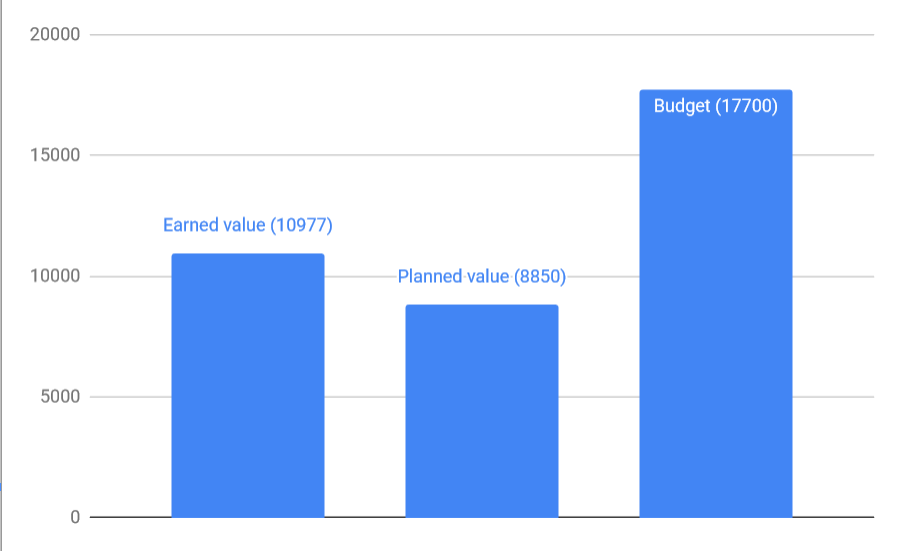
\includegraphics[width=10cm,keepaspectratio]{../includes/pics/SV.PNG}
	\caption{\label{fig:mission}Schedule variance}
\end{figure}
\begin{figure}[H]
	\centering
	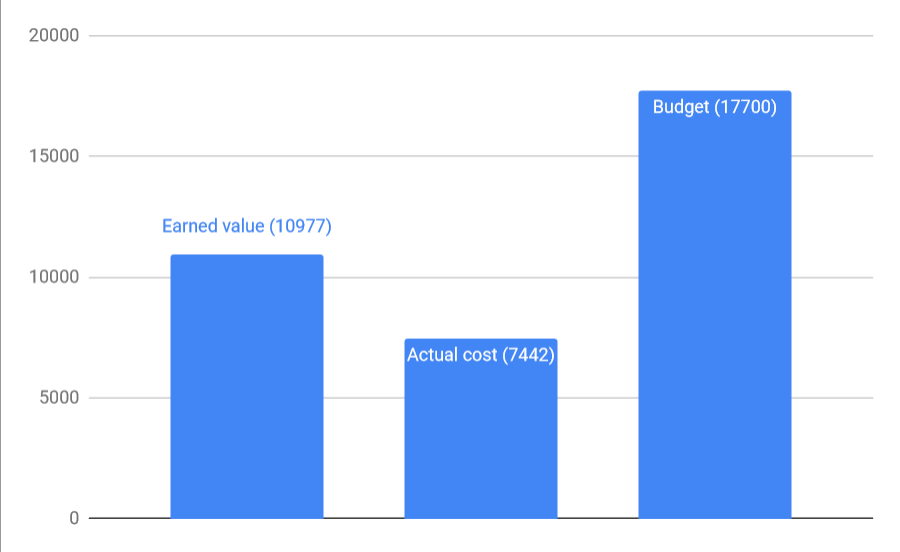
\includegraphics[width=10cm,keepaspectratio]{../includes/pics/BV.PNG}
	\caption{\label{fig:mission}Budget variance}
\end{figure}
\paragraph{MPRDP003 - Rischi non previsti}\mbox{}\\[0.4cm]
I rischi presentatisi in questa fase sono tutti già individuati nel set dei rischi. Di conseguenza non viene riportato alcun rischio non preventivato.
\paragraph{MPRDP004 - Indisponibilità servizi terzi}\mbox{}\\[0.4cm]
I servizi terzi utilizzati non hanno subito interruzioni di disponibilità in nessun periodo. Di conseguenza non viene riportata alcuna segnalazione.
\paragraph{MPRDP005 - Media di commit per settimana}\mbox{}\\[0.4cm]
Nella tabella sottostante è mostrato il risultato ottenuto per le repository utilizzate.
\begin{center}%%TODO aggiorna numeri
	\centering
	\renewcommand{\arraystretch}{1.5}
	\rowcolors{3}{tableLightYellow}{}
	\begin{longtable}{  p{5cm}  p{5cm} }
		\rowcolor{tableHeadYellow}
		\textbf{Repository}   & \textbf{N. commit settimanali} \\ 
		\endhead
		Documenti    &           90                      \\
		Applicazione Android         & 9             \\
		Backend AWS    & 20                           \\
		\rowcolor{white}
		\caption{Resoconto misurazioni metrica MPRDP005 - Media commit per settimana}
	\end{longtable}
\end{center}
\subsubsection{Documenti}
\paragraph{MPRDD001 - Indice di Gulpease}\mbox{}\\[0.4cm]
Per mezzo di script automatici è stato possibile istanziare la metrica  \textbf{MPRDD001 Indice di Gulpease}.\\
Nella tabella sottostante è mostrato il risultato ottenuto per i principali documenti prodotti.
\begin{center}%%TODO aggiorna numeri
	\centering
	\renewcommand{\arraystretch}{1.5}
	\rowcolors{3}{tableLightYellow}{}
	\begin{longtable}{  p{5cm}  p{5cm} p{3cm}  }
		\rowcolor{tableHeadYellow}
		\textbf{Nome documento}   & \textbf{Indice di \mbox{Gulpease}} & \textbf{Esito} \\ 
		\endhead
		Studio di Fattibilità     & 89                                 & Ottimo \\
		Norme di Progetto         & 83                                 & Ottimo \\
		Analisi dei Requisiti     & 81                                 & Ottimo \\
		Piano di Progetto         & 84                                & Ottimo \\
		Piano di Qualifica        & 90                                 & Ottimo \\
		\rowcolor{white}
		\caption{Resoconto misurazioni metrica MPRDD001 - Indice di Gulpease}
	\end{longtable}
\end{center}
\paragraph{MPRDD002 - Errori ortografici}\mbox{}\\[0.4cm]
Tutti i documenti, dopo un rigoroso controllo da parte dei verificatori ed un feedback positivo rilasciato dallo strumento di controllo della sintassi di TexStudio, risultano privi di errori e raggiungono il valore accettabile ed ottimale della metrica  \textbf{MPRDD002 Correttezza ortografica}.
\clearpage
\subsubsection{Software}
\paragraph{MPRDS001 - Copertura requisiti obbligatori}\mbox{}\\[0.4cm]
Sono coperti da implementazione il 62\% dei requisiti obbligatori.
\paragraph{MPRDS002 - Copertura requisiti accettati}\mbox{}\\[0.4cm]
Sono coperti da implementazione il 22\% dei requisiti accettati.
%%ds 4 5 e 6 non sono ancora misurabili
\paragraph{MPRDS009 - Complessità ciclomatica}\mbox{}\\[0.4cm]
La misura è stata effettuata tramite il plugin CodeMR. Per il codice dell' applicazione Android, su un totale di 24 classi, sono state individuate: \begin{itemize}
\item 7 classi di complessità bassa (verde scuro)
\item 8 classi di complessità medio-bassa (verde chiaro)
\item 6 classi di complessità medio-alta (giallo)
\end{itemize}
\begin{figure}[H]
	\centering
	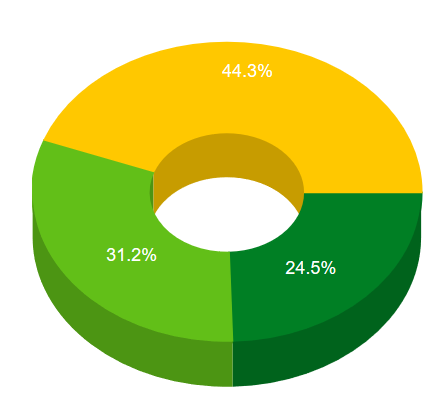
\includegraphics[width=10cm,keepaspectratio]{../includes/pics/complexity.PNG}
	\caption{\label{fig:mission}MPRDS009 - Complessità ciclomatica}
\end{figure}
%%la figura è in pics domani faccio
\paragraph{MPRDS010 - Numero di metodi}\mbox{}\\[0.4cm]
\begin{itemize}
\item La parte Android dell'Applicazione conta di 61 metodi.
\item La parte AWS Lambda dell'Applicazione conta di 85 metodi.
\end{itemize}

%chiedi a chi di competenza 
\paragraph{MPRDS011 - Variabili non utilizzate}\mbox{}\\[0.4cm]
Le variabili inutilizzate sono segnalate come warnings dagli IDE utilizzati, sono perciò facili da individuare, il loro valore è 0.
\subsubsection{Test sul software}
I risultati sono relativi allo stato attuale di Revisione di Progettazione, sono stati applicati pochi test per l'applicazione Android, solo quelli necessari a coprire i requisiti necessari ad un proof of concept, per quanto riguarda il backend AWS Lambda i test sono automaticamente generati per ogni Lambda implementata. Non è ancora stato definito il numero totale di test che si andranno ad eseguire, questo numero sarà molto vicino al numero totale di requisiti definiti in analisi dei requisiti.
\paragraph{MPRC006 - Misurazione dei test}\mbox{}\\[0.4cm]
\begin{center}
	\centering
	\renewcommand{\arraystretch}{1.5}
	\rowcolors{3}{tableLightYellow}{}
	\begin{longtable}{  p{5cm}  p{5cm} p{3cm}  }
		\rowcolor{tableHeadYellow}
		\textbf{Metrica}   & \textbf{Valore ottenuto} & \textbf{Esito} \\ 
		\endhead
		Percentuale test passati     & 100\%  & Ottimale \\
		Percentuale test falliti     & 0\% & Ottimale \\
		Efficienza progettazione test    & 25 minuti & Accettabile \\
		Contenimento dei difetti    & 80\% & Accettabile \\
		\rowcolor{white}
		\caption{Resoconto misurazioni metrica MPRC006 - Misurazione dei test}
	\end{longtable}
\end{center}
\clearpage
\subsection{Revisione di Qualifica}
\label{sec:revisione_qualifica}
La sezione verrà implementata alla fine del periodo indicato.
\subsection{Revisione di Accettazione}
\label{sec:revisione_accettazione}
La sezione verrà implementata alla fine del periodo indicato.
